\documentclass[12pt]{article}

\usepackage[russian]{babel}
\usepackage{amssymb}
\usepackage{amsmath}
\usepackage{mathrsfs}
\usepackage[pdftex]{graphicx}

\title{Изменение траектории частицы при увеличении электрического поля.}
\author {}
\date{}

\begin{document}

ыыыыыыФБВТ

СКОЛКОВО РУЛИТ 

$$x_{n+1}^2 = \sqrt{2 + x_n}$$

$$f(x) = \int\limits_{34}^{47}\frac{x+1}{x^2 + 3x + 2}dx = 555$$

На картинке \ref{2__} можно видеть рыбок.

\begin{figure}[h]\center
{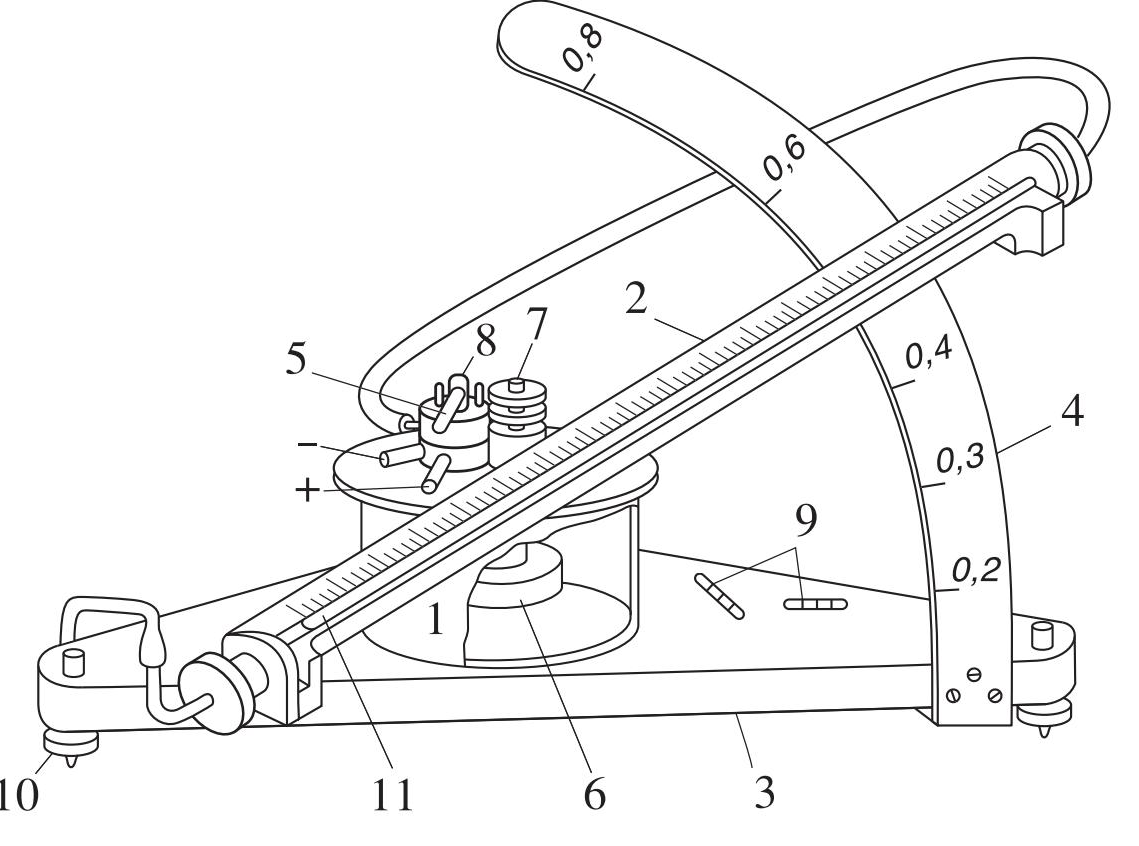
\includegraphics[width=150mm]{2.png}}
\caption{ЭТО РЫБКИ}

\label{2__}
\end{figure}




\end{document}